\documentclass[14pt,aspectratio=169]{beamer}

\usepackage{amssymb, amsmath}
%\usepackage[all]{xy}

\usepackage{alltt}
\usepackage{pslatex}
\usepackage{epigraph}
\usepackage{verbatim}

\usepackage{url}

%\usepackage{graphicx}
\usepackage{latexsym}
\usepackage{array}
\usepackage{comment}
\usepackage{makeidx}
\usepackage{listings}
\usepackage{indentfirst}
\usepackage{verbatim}
\usepackage{color}
\usepackage{url}
\usepackage{xspace}
%\usepackage{fontspec}
%\usepackage{xunicode}
%\usepackage{xltxtra}
%\usepackage{xecyr}
\usepackage{hyperref}
%\usepackage[english]{babel}
%\usepackage[utf8]{inputenc}
%\setmainfont[Mapping=tex-text]{DejaVu Serif}
%\setsansfont[Mapping=tex-text]{DejaVu Sans}
%\setmonofont[Mapping=tex-text]{DejaVu Sans Mono}
%\usepackage{polyglossia}
%\setdefaultlanguage{russian}
\usepackage{stmaryrd}

\usepackage{amsmath, amsthm, amssymb}
\usepackage{graphicx}
\usepackage{euscript}
\usepackage{mathtools}
\usepackage{xcolor}
\usepackage{multirow}
\usepackage{pgfplots}

\makeatletter
\begin{comment}
\newcolumntype{e}[1]{%--- Enumerated cells ---
   >{\minipage[t]{\linewidth}%
     \NoHyper%                Hyperref adds a vertical space
     \let\\\tabularnewline
     \enumerate
        \addtolength{\rightskip}{0pt plus 50pt}% for raggedright
        \setlength{\itemsep}{-\parsep}}%
   p{#1}%
   <{\@finalstrut\@arstrutbox\endenumerate
     \endNoHyper
     \endminipage}}

\newcolumntype{i}[1]{%--- Itemized cells ---
   >{\minipage[t]{\linewidth}%
        \let\\\tabularnewline
        \itemize
           \addtolength{\rightskip}{0pt plus 50pt}%
           \setlength{\itemsep}{-\parsep}}%
   p{#1}%
   <{\@finalstrut\@arstrutbox\enditemize\endminipage}}

\AtBeginDocument{%
    \@ifpackageloaded{hyperref}{}%
        {\let\NoHyper\relax\let\endNoHyper\relax}}
\end{comment}

\makeatother

\definecolor{shadecolor}{gray}{1.00}
\definecolor{darkgray}{gray}{0.30}

\newcommand{\set}[1]{\{#1\}}
\newcommand{\angled}[1]{\langle {#1} \rangle}
\newcommand{\fib}{\rightarrow_{\mathit{fib}}}
\newcommand{\fibm}{\Rightarrow_{\mathit{fib}}}
\newcommand{\oo}[1]{${#1}^o$}
\newcommand{\inml}[1]{\mbox{\lstinline{#1}}}
\newcommand{\goal}{\mathfrak G}
\newcommand{\inmath}[1]{\mbox{$#1$}}
\newcommand{\sembr}[1]{\llbracket{#1}\rrbracket}

\newcommand{\withenv}[2]{{#1}\vdash{#2}}
\newcommand{\ruleno}[1]{\mbox{[\textsc{#1}]}}
\newcommand{\trule}[2]{\dfrac{#1}{#2}}

%\setlength{\epigraphwidth}{.55\textwidth}

\definecolor{light-gray}{gray}{0.90}
\newcommand{\graybox}[1]{\colorbox{light-gray}{#1}}

\newcommand{\nredrule}[3]{
  \begin{array}{cl}
    \textsf{[{#1}]}&
    \begin{array}{c}
      #2 \\
      \hline
      \raisebox{-1pt}{\ensuremath{#3}}
    \end{array}
  \end{array}}

\newcommand{\naxiom}[2]{
  \begin{array}{cl}
    \textsf{[{#1}]} & \raisebox{-1pt}{\ensuremath{#2}}
  \end{array}}

\definecolor{myRed}{rgb}{0.5, 0, 0}
\definecolor{myBlue}{rgb}{0, 0, 0.6}

\lstdefinelanguage{ocaml}{
keywords={let, begin, end, in, match, type, and, fun,
function, try, with, class, object, method, of, rec, until,
while, not, do, done, as, val, inherit, module, sig, @type, struct,
if, then, else, open, virtual, new, fresh, conde, run},
sensitive=true,
basicstyle=\small,
commentstyle=\scriptsize\rmfamily,
keywordstyle=\ttfamily\bfseries,
identifierstyle=\ttfamily,
basewidth={0.5em,0.5em},
columns=fixed,
fontadjust=true,
moredelim=**[is][\ttfamily]{~}{~},
moredelim=**[is][\color{myRed}]{@}{@},
moredelim=**[is][\color{myBlue}]{<}{>},
literate={fun}{{$\lambda$}}1 {->}{{$\to$}}3 {===}{{$\equiv$}}1 {=/=}{{$\not\equiv$}}1 {|>}{{$\triangleright$}}3 {\&\&\&}{{$\wedge$}}2 {|||}{{$\vee$}}2 {^}{{$\uparrow$}}1,
morecomment=[s]{(*}{*)}
}

\lstset{
mathescape=true,
basicstyle=\small,
identifierstyle=\ttfamily,
keywordstyle=\bfseries,
commentstyle=\scriptsize\rmfamily,
basewidth={0.5em,0.5em},
fontadjust=true,
escapechar=!,
language=ocaml
}

\begin{comment}
\lstdefinelanguage{ocaml}{
keywords={fresh, let, begin, end, in, match, type, and, fun, function, try, with, when, class,
object, method, of, rec, until, while, not, do, done, as, val, inherit,
new, module, sig, deriving, datatype, struct, if, then, else, open, private, virtual, include, @type},
sensitive=true,
commentstyle=\small\itshape\ttfamily,
keywordstyle=\ttfamily\underbar,
identifierstyle=\ttfamily,
basewidth={0.5em,0.5em},
columns=fixed,
fontadjust=true,

literate={->}{{$\to\;\;$}}3 {===}{{$\equiv$}}3 {=/=}{{$\not\equiv$}}3 {|>}{{$\triangleright$}}3,
morecomment=[s]{(*}{*)}
}

\lstset{
mathescape=true,
identifierstyle=\ttfamily,
keywordstyle=\bfseries,
commentstyle=\scriptsize\rmfamily,
basewidth={0.5em,0.5em},
fontadjust=true,
language=ocaml
}
\end{comment}
\sloppy

\newcommand{\miniKanren}{\texttt{miniKanren}\xspace}
\newcommand{\ocanren}{\texttt{OCanren}\xspace}
\newcommand{\ocaml}{\texttt{OCaml}\xspace}
\newcommand{\mk}{\texttt{miniKanren}\xspace}
\newcommand{\inbr}[1]{\langle #1 \rangle}
\renewcommand{\emptyset}{\varnothing}

\setbeamertemplate{footline}[frame number]
\setbeamertemplate{navigation symbols}{}
\setbeamertemplate{blocks}[rounded][shadow=true]
\beamertemplateballitem

\mode<presentation>{
  \usetheme{default}
}

\theoremstyle{definition}

\title{On Fair Conjunction
}


\author{
 \underline{Petr Lozov} \and Dmitry Boulytchev
}

\institute[]{
\small{
\textbf{Saint Petersburg State University $\: $\\JetBrains Research}
}
}

\date{
   \vskip 1cm
   \small{
   \textbf{miniKanren workshop}\\
   August 27, 2020\
  }
}

\begin{document}

\begin{frame}[plain]
  \titlepage
\end{frame}

\begin{frame}[fragile]{Conjunction in ~\!\mk}
Operation to find common answers for several goals
\vskip5mm
\begin{itemize}
  \item[$\bullet$] Left-biased operation
  \vskip3mm
  \item[$\bullet$] The order of conjuncts doesn't affect search completeness
  \vskip4mm
  \item[$\bullet$] The order of conjuncts affects
  \begin{itemize}
    \normalsize
    \item[$\circ$] Performance
    \item[$\circ$] Convergence
  \end{itemize}
\end{itemize}
\end{frame}

\begin{frame}[fragile]{Example}
\begin{center}
\begin{tabular}{cp{5mm}|p{5mm}c}
\begin{lstlisting}
let sort$^o$ x y = conde [
  x === [] &&& y === [];
  fresh (a xs ys)
    (y === a :: ys)
    (~@smallest$^{\textcolor{myRed}{o}}$ x a xs@~)
    (~<sort$^{\textcolor{myBlue}{o}}$ xs ys>~)]
\end{lstlisting} &&&
\begin{lstlisting}
let sort$^o$ x y = conde [
  x === [] &&& y === [];
  fresh (a xs ys)
    (y === a :: ys)
    (~<sort$^{\textcolor{myBlue}{o}}$ xs ys>~)
    (~@smallest$^{\textcolor{myRed}{o}}$ x a xs@~)]
\end{lstlisting} \pause
\\[5mm] &&&
\\[5mm]
\begin{lstlisting}
 run$^*$ q (sort$^o$ [4;3;2;1] q) $$
\end{lstlisting} &&&
\begin{lstlisting}
 run$^*$ q (sort$^o$ [4;3;2;1] q) $$
\end{lstlisting}\\
$\downarrow$ &&& $\downarrow$ \\
\begin{lstlisting}
[q = [1;2;3;4]]
\end{lstlisting}
&&&
\begin{lstlisting}
[q = [1;2;3;4]; ...
\end{lstlisting} \\ &&&
\end{tabular}
\end{center}
\end{frame}

\begin{frame}[fragile, noframenumbering]{Example}
\begin{center}
\begin{tabular}{cp{5mm}|p{5mm}c}

\begin{lstlisting}
let sort$^o$ x y = conde [
  x === [] &&& y === [];
  fresh (a xs ys)
    (y === a :: ys)
    (~@smallest$^{\textcolor{myRed}{o}}$ x a xs@~)
    (~<sort$^{\textcolor{myBlue}{o}}$ xs ys>~)]
\end{lstlisting} &&&
\begin{lstlisting}
let sort$^o$ x y = conde [
  x === [] &&& y === [];
  fresh (a xs ys)
    (y === a :: ys)
    (~<sort$^{\textcolor{myBlue}{o}}$ xs ys>~)
    (~@smallest$^{\textcolor{myRed}{o}}$ x a xs@~)]
\end{lstlisting}
\\[5mm] &&&
\\[5mm]
\begin{lstlisting}
 run$^1$ q (sort$^o$ [4;3;2;1] q) $$
\end{lstlisting} &&&
\begin{lstlisting}
 run$^1$ q (sort$^o$ [4;3;2;1] q) $$
\end{lstlisting} \\
$\downarrow$ &&& $\downarrow$ \\
\begin{lstlisting}
[q = [1;2;3;4]]
\end{lstlisting}
&&&
\begin{lstlisting}
[q = [1;2;3;4]]
\end{lstlisting} \\
{\small (0.424s)} &&&
{\small (3.924s)}
\end{tabular}
\end{center}
\end{frame}

\begin{frame}[fragile, noframenumbering]{Example}
\begin{center}
\begin{tabular}{cp{5mm}|p{5mm}c}

\begin{lstlisting}
let sort$^o$ x y = conde [
  x === [] &&& y === [];
  fresh (a xs ys)
    (y === a :: ys)
    (~@smallest$^{\textcolor{myRed}{o}}$ x a xs@~)
    (~<sort$^{\textcolor{myBlue}{o}}$ xs ys>~)]
\end{lstlisting} &&&
\begin{lstlisting}
let sort$^o$ x y = conde [
  x === [] &&& y === [];
  fresh (a xs ys)
    (y === a :: ys)
    (~<sort$^{\textcolor{myBlue}{o}}$ xs ys>~)
    (~@smallest$^{\textcolor{myRed}{o}}$ x a xs@~)]
\end{lstlisting}
\\[5mm] &&&
\\[5mm]
\begin{lstlisting}
run$^1$ q (sort$^o$ [5;4;3;2;1] q)
\end{lstlisting} &&&
\begin{lstlisting}
run$^1$ q (sort$^o$ [5;4;3;2;1] q)
\end{lstlisting} \\
$\downarrow$ &&& $\downarrow$ \\
\begin{lstlisting}
[q = [1;2;3;4;5]]
\end{lstlisting}
&&&
\begin{lstlisting}
(???)
\end{lstlisting} \\
{\small (0.430s)} &&&
{\small ($>$300s)}
\end{tabular}
\end{center}
\end{frame}

\begin{frame}[fragile]{Fair Conjunction}
\centering

$g_1 \; \land \; g_2$ converges $\;\Leftrightarrow\;$ $g_2 \; \land \; g_1$ converges

\vskip1cm
\textbf{Goal} \\
Introduce fair conjunction into \mk

\end{frame}

\begin{frame}[fragile]{From Disjunction to Conjunction}
\begin{center}
    \mk disjunction is fair due to \emph{interleaving} search
    \vskip1cm
    Disjunction interleaves evaluation steps of disjuncts
    \vskip1cm
    Let's try to interleave evaluation steps of conjuncts
\end{center}
\end{frame}

\begin{frame}[fragile]{Naive Fair Conjunction Algorithm}

\begin{center}
\emph{Unfolding bound} $\textcolor{myRed}{N}$ is parameter of algorithm
\end{center}
\vskip5mm
\begin{itemize}
    \item[$\bullet$] Conjuncts are unfolded from left to right
    \item[$\bullet$] Each conjunt is unfolded no more than $\textcolor{myRed}{N}$ times
    \item[$\bullet$] If all conjuncts was unfolded $\textcolor{myRed}{N}$ times, then again go to the leftmost conjunct
\end{itemize}
\end{frame}


\begin{frame}[fragile]{Example}
\begin{center}
\begin{tabular}{cp{5mm}|p{5mm}c}

\begin{lstlisting}
let sort$^o$ x y = conde [
  x === [] &&& y === [];
  fresh (a xs ys)
    (y === a :: ys)
    (~@smallest$^{\textcolor{myRed}{o}}$ x a xs@~)
    (~<sort$^{\textcolor{myBlue}{o}}$ xs ys>~)]
\end{lstlisting} &&&
\begin{lstlisting}
let sort$^o$ x y = conde [
  x === [] &&& y === [];
  fresh (a xs ys)
    (y === a :: ys)
    (~<sort$^{\textcolor{myBlue}{o}}$ xs ys>~)
    (~@smallest$^{\textcolor{myRed}{o}}$ x a xs@~)]
\end{lstlisting}
\\[5mm] &&&
\\[5mm]
\begin{lstlisting}
run$^*$ q (sort$^o$ [5;4;3;2;1] q)
\end{lstlisting} &&&
\begin{lstlisting}
run$^*$ q (sort$^o$ [5;4;3;2;1] q)
\end{lstlisting} \\
$\qquad\quad$ $\downarrow$ $\scriptstyle (\textcolor{myRed}{N} = 100)$ &&&
$\qquad\;\;$ $\downarrow$ $\scriptstyle (\textcolor{myRed}{N} = 11)$ \\
\begin{lstlisting}
[q = [1;2;3;4;5]]
\end{lstlisting}
&&&
\begin{lstlisting}
[q = [1;2;3;4;5]]
\end{lstlisting} \\
{\small (0.428s)} &&&
{\small (0.969s)}
\end{tabular}
\end{center}
\end{frame}

\begin{frame}[fragile]{Naive Fair Conjunction}
\begin{itemize}
    \item[$\boldsymbol{+}$] Better convergence than left-biased conjunction
    \vskip3mm
    \item[$\boldsymbol{+}$] Better performance at matched \emph{unfolding bound} $\textcolor{myRed}{N}$
    \vskip3mm
    \item[$\boldsymbol{-}$] Optimal $\textcolor{myRed}{N}$ must be selected for each program
    \vskip3mm
    \item[$\boldsymbol{-}$]  $\textcolor{myRed}{N}$ is common for all conjuncts
    \vskip3mm
    \item[$\boldsymbol{-}$] First conjunct switching is after $\textcolor{myRed}{N}$ steps
\end{itemize}
\end{frame}

\begin{frame}[fragile]{Dynamic Unfolding Bound}
\begin{center}
    \emph{Unfolding predicate} $\textcolor{myRed}{pred}$ determines when to reorder conjuncts
\end{center}
$$\textcolor{myRed}{pred} : Substs \times Calls \rightarrow \set{\bot; \top}$$
\begin{itemize}
    \item[$\bullet$] $\top \Leftrightarrow$ continue conjunct evaluation
    \item[$\bullet$] $\bot \Leftrightarrow$ stop conjunct evaluation and go to another conjunct
\end{itemize}
\end{frame}



\begin{frame}[fragile]{Structural Recursion}
\begin{center}
Relation argument $x$ is structural recursive if it structurally decreases with each recursion step
\vskip1cm
Relation is structural recursive if it has at least one structural recursive argument
\end{center}
\end{frame}

\begin{frame}[fragile]{Structural Recursion: Example}
\begin{tabular}{cc}
\begin{lstlisting}
let rec append$^o$ x y z =
  (x === [] &&& y === z) |||
  fresh (e xs zs)
    (x === e : xs)
    (z === e : zs)
    (append$^o$ xs y zs)
\end{lstlisting} &
\begin{tabular}{c}
\lstinline|x| is structural recursive argument \\[5mm]
\lstinline|z| is structural recursive argument \\[5mm]
\lstinline|append$^o$| is structural recursion relation
\end{tabular}
\end{tabular}
\end{frame}

\begin{frame}[fragile]{Structural Recursion: Predicate}

\centering
Structural recursive relation diverges if all of its structural arguments are free variables

\[
pred(\sigma, F^k(t_1, \ldots, t_k)) = \left\{
\begin{array}{cl}
      & \mbox{if } F \mbox{ is structural recursive relation, } \\
\top, & t_i \mbox { is structural recursive argument, } \\
      & t_i \mbox { is not fresh variable in } \sigma \\
\bot, & \mbox{otherwise.}
\end{array}
\right.
\]
\end{frame}

\begin{frame}[fragile]{Fair Conjunction by Structural Recursion Algorithm}
\begin{center}
\emph{Unfolding predicate} $\textcolor{myRed}{pred}$ is parameter of algorithm
\end{center}
$$\textcolor{myRed}{pred} : Substs \times Calls \rightarrow \set{\bot; \top}$$
\vskip5mm
\begin{itemize}

    \item[$\bullet$] Conjuncts are unfolded from left to right
    \item[$\bullet$] Each conjunt is unfolded while $\textcolor{myRed}{pred}$ is $\top$
    \item[$\bullet$] If $\textcolor{myRed}{pred}$ is $\bot$ for all conjunts we use naive fair conjunction behavior

\end{itemize}
\end{frame}

\begin{frame}[fragile, noframenumbering]{Example}
\begin{center}
\begin{tabular}{cp{5mm}|p{5mm}c}

\begin{lstlisting}
let sort$^o$ x y = conde [
  x === [] &&& y === [];
  fresh (a xs ys)
    (y === a :: ys)
    (~@smallest$^{\textcolor{myRed}{o}}$ x a xs@~)
    (~<sort$^{\textcolor{myBlue}{o}}$ xs ys>~)]
\end{lstlisting} &&&
\begin{lstlisting}
let sort$^o$ x y = conde [
  x === [] &&& y === [];
  fresh (a xs ys)
    (y === a :: ys)
    (~<sort$^{\textcolor{myBlue}{o}}$ xs ys>~)
    (~@smallest$^{\textcolor{myRed}{o}}$ x a xs@~)]
\end{lstlisting}
\\[5mm] &&&
\\[5mm]
\begin{lstlisting}
 run$^1$ q (sort$^o$ [5;4;3;2;1] q) $$
\end{lstlisting} &&&
\begin{lstlisting}
 run$^1$ q (sort$^o$ [5;4;3;2;1] q) $$
\end{lstlisting} \\
$\downarrow$ &&& $\downarrow$ \\
\begin{lstlisting}
[q = [1;2;3;4;5]]
\end{lstlisting}
&&&
\begin{lstlisting}
[q = [1;2;3;4;5]]
\end{lstlisting} \\
{\small (0.433s)} &&&
{\small (0.432s)}
\end{tabular}
\end{center}
\end{frame}

\begin{frame}[fragile]{Fair Conjunction by Structural Recursion}
\begin{itemize}
    \item[$\boldsymbol{+}$] Same convergence as naive fair conjunction
    \vskip3mm
    \item[$\boldsymbol{+}$] Better performance than left-biased and naive fair conjunctions
    \vskip3mm
    \item[$\boldsymbol{+}$] Instant switching of conjuncts in case of divergence
    \vskip3mm
    \item[$\boldsymbol{-}$] If relation is without structural recursion it becomes naive fair conjunction
\end{itemize}
\end{frame}

\begin{frame}[fragile]{Evaluation: Optimistic Case}
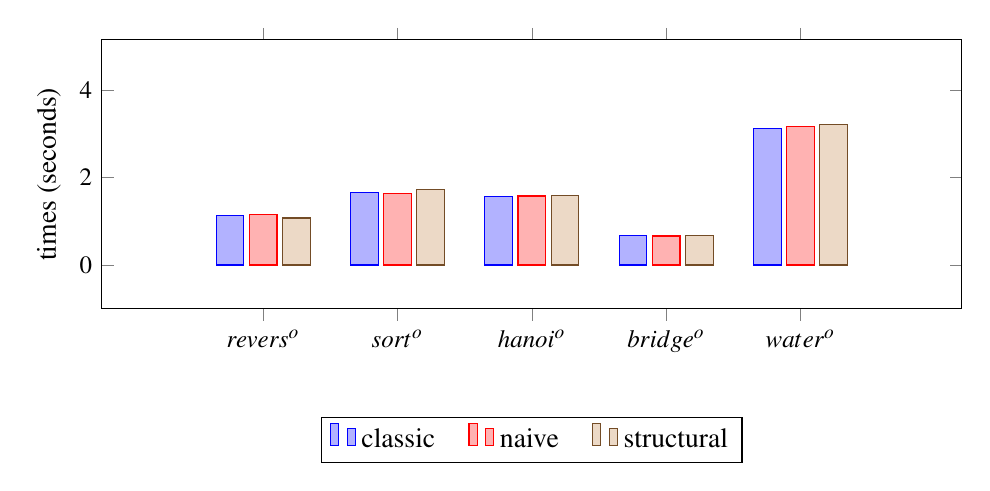
\begin{tikzpicture}
\begin{axis}[
    ybar, ymax = 4, ymin = 0.15,
    enlargelimits=0.3,
    width=125mm, height=5cm,
    legend style={at={(0.5,-0.4)},
      anchor=north,legend columns=-1},
    ylabel={times (seconds)},
    tick label style={font=\small},
    symbolic x coords={$revers^o$, $sort^o$, $hanoi^o$, $bridge^o$, $water^o$},
    xtick=data
    ]
\addplot coordinates {($revers^o$,1.142) ($sort^o$,1.664) ($hanoi^o$,1.574) ($bridge^o$,0.669) ($water^o$,3.132)};
\addplot coordinates {($revers^o$,1.151) ($sort^o$,1.636) ($hanoi^o$,1.579) ($bridge^o$,0.663) ($water^o$,3.168)};
\addplot coordinates {($revers^o$,1.077) ($sort^o$,1.723) ($hanoi^o$,1.585) ($bridge^o$,0.675) ($water^o$,3.220)};
\legend{classic$\quad$,naive$\quad$,structural}
\end{axis}
\end{tikzpicture}
\end{frame}

\begin{frame}[fragile]{Evaluation: Pessimistic Case}
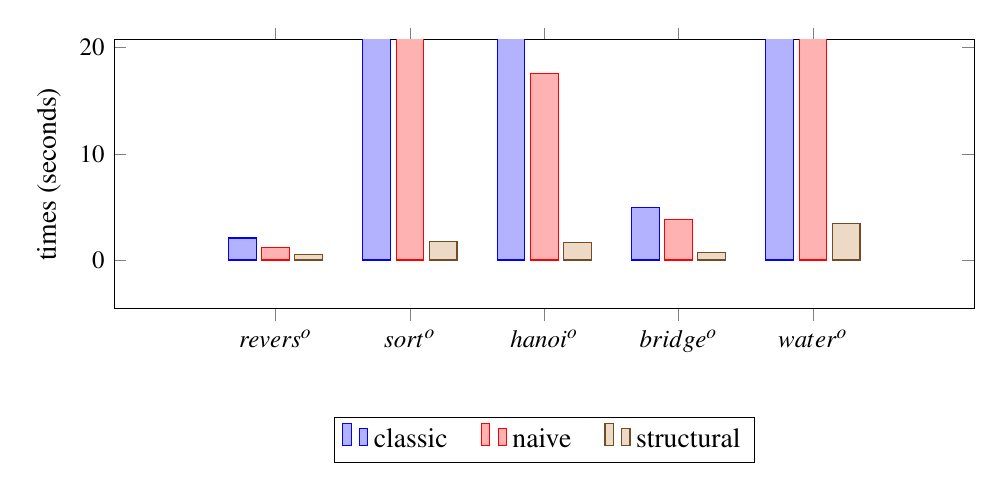
\begin{tikzpicture}
\begin{axis}[
    ybar, ymax = 16, ymin = 0.15,
    enlargelimits=0.3,
    width=125mm, height=5cm,
    legend style={at={(0.5,-0.4)},
      anchor=north,legend columns=-1},
    ylabel={times (seconds)},
    tick label style={font=\small},
    symbolic x coords={$revers^o$, $sort^o$, $hanoi^o$, $bridge^o$, $water^o$},
    xtick=data
    ]
\addplot coordinates {($revers^o$,2.073) ($sort^o$,300) ($hanoi^o$,300) ($bridge^o$,4.956) ($water^o$,300)};
\addplot coordinates {($revers^o$,1.151) ($sort^o$,300) ($hanoi^o$,17.604) ($bridge^o$,3.820) ($water^o$,300)};
\addplot coordinates {($revers^o$,0.542) ($sort^o$,1.751) ($hanoi^o$,1.646) ($bridge^o$,0.712) ($water^o$,3.414)};
\legend{classic$\quad$,naive$\quad$,structural}
\end{axis}
\end{tikzpicture}
\end{frame}

\begin{frame}[fragile]{More in the Paper}
\begin{itemize}
     \item[$\bullet$] Another one formal semantics for \mk with directed conjunction
    \vskip5mm
    \item[$\bullet$] Two formal semantics for \mk with fair conjunction
    \vskip5mm
    \item[$\bullet$] Evaluation of all three semantics
\end{itemize}
\end{frame}

\begin{frame}[fragile]{Future Work}
\begin{itemize}
    \item[$\bullet$] Generalize our approach to larger class of programs
    \vskip5mm
    \item[$\bullet$] Formalize our approach in Coq proof assistant
    \vskip5mm
    \item[$\bullet$] Formally prove equivalence with denotational semantics
    \vskip5mm
    \item[$\bullet$] Formally prove conjunction fairness
\end{itemize}
\end{frame}



\begin{frame}
\begin{center}
{\Huge Thanks!}
\end{center}
\end{frame}

\end{document}
